\iffalse
This file is protected by Copyright. Please refer to the COPYRIGHT file
distributed with this source distribution.

This file is part of OpenCPI <http://www.opencpi.org>

OpenCPI is free software: you can redistribute it and/or modify it under the
terms of the GNU Lesser General Public License as published by the Free Software
Foundation, either version 3 of the License, or (at your option) any later
version.

OpenCPI is distributed in the hope that it will be useful, but WITHOUT ANY
WARRANTY; without even the implied warranty of MERCHANTABILITY or FITNESS FOR A
PARTICULAR PURPOSE. See the GNU Lesser General Public License for more details.

You should have received a copy of the GNU Lesser General Public License along
with this program. If not, see <http://www.gnu.org/licenses/>.
\fi
%----------------------------------------------------------------------------------------
% Update the docTitle and docVersion per document
%----------------------------------------------------------------------------------------
\def\docTitle{Debugging Tools Guide}
\def\docVersion{1.4}
%----------------------------------------------------------------------------------------
\documentclass{article}
\iffalse
This file is protected by Copyright. Please refer to the COPYRIGHT file
distributed with this source distribution.

This file is part of OpenCPI <http://www.opencpi.org>

OpenCPI is free software: you can redistribute it and/or modify it under the
terms of the GNU Lesser General Public License as published by the Free Software
Foundation, either version 3 of the License, or (at your option) any later
version.

OpenCPI is distributed in the hope that it will be useful, but WITHOUT ANY
WARRANTY; without even the implied warranty of MERCHANTABILITY or FITNESS FOR A
PARTICULAR PURPOSE. See the GNU Lesser General Public License for more details.

You should have received a copy of the GNU Lesser General Public License along
with this program. If not, see <http://www.gnu.org/licenses/>.
\fi
\author{} % Force author to be blank
%----------------------------------------------------------------------------------------
% Paper size, orientation and margins
%----------------------------------------------------------------------------------------
\usepackage{geometry}
\geometry{
        letterpaper, % paper type
        portrait,    % text direction
        left=.75in,  % left margin
        top=.75in,   % top margin
        right=.75in, % right margin
        bottom=.75in % bottom margin
 }
%----------------------------------------------------------------------------------------
% Header/Footer
%----------------------------------------------------------------------------------------
\usepackage{fancyhdr} \pagestyle{fancy} % required for fancy headers
\renewcommand{\headrulewidth}{0.5pt}
\renewcommand{\footrulewidth}{0.5pt}
\rhead{\small{ANGRYVIPER Team}}
% \rfoot{\thepage}
%----------------------------------------------------------------------------------------
% Appendix packages
%----------------------------------------------------------------------------------------
\usepackage[toc,page]{appendix}
%----------------------------------------------------------------------------------------
% Defined Commands & Renamed Commands
%----------------------------------------------------------------------------------------
\renewcommand{\contentsname}{Table of Contents}
\renewcommand{\listfigurename}{List of Figures}
\renewcommand{\listtablename}{List of Tables}
%----------------------------------------------------------------------------------------
% Various packages
%----------------------------------------------------------------------------------------
\usepackage[usenames,dvipsnames]{xcolor} % for color names see https://en.wikibooks.org/wiki/LaTeX/Colors
\usepackage{hyperref}  % for linking urls and lists
\usepackage{graphicx}  % for including pictures by file
\usepackage{listings}  % for coding language styles
\usepackage{rotating}  % for sideways table
\usepackage{pifont}    % for sideways table
\usepackage{pdflscape} % for landscape view
\usepackage{subfig}
\usepackage{xstring}
\uchyph=0 % Never hyphenate acronyms like RCC (I think this overrides ANGRYVIPER above)
\renewcommand\_{\textunderscore\allowbreak} % Allow words to break/newline on underscores
%----------------------------------------------------------------------------------------
% Table packages
%----------------------------------------------------------------------------------------
\usepackage{longtable} % for long possibly multi-page tables
\usepackage{tabularx} % c=center,l=left,r=right,X=fill
% These define tabularx columns "C" and "R" to match "X" but center/right aligned
\newcolumntype{C}{>{\centering\arraybackslash}X}
\newcolumntype{R}{>{\raggedleft\arraybackslash}X}
\usepackage{float}
\floatstyle{plaintop}
\usepackage[tableposition=top]{caption}
\newcolumntype{P}[1]{>{\centering\arraybackslash}p{#1}}
\newcolumntype{M}[1]{>{\centering\arraybackslash}m{#1}}
%----------------------------------------------------------------------------------------
% Block Diagram / FSM Drawings
%----------------------------------------------------------------------------------------
\usepackage{tikz}
\usetikzlibrary{shapes,arrows,fit,positioning}
\usetikzlibrary{automata} % used for the fsm
%----------------------------------------------------------------------------------------
% Colors Used
%----------------------------------------------------------------------------------------
\usepackage{colortbl}
\definecolor{blue}{rgb}{.7,.8,.9}
\definecolor{ceruleanblue}{rgb}{0.16, 0.32, 0.75}
\definecolor{drkgreen}{rgb}{0,0.6,0}
\definecolor{deepmagenta}{rgb}{0.8, 0.0, 0.8}
\definecolor{cyan}{rgb}{0.0,0.6,0.6}
\definecolor{maroon}{rgb}{0.5,0,0}
%----------------------------------------------------------------------------------------
% VHDL Coding Language Style
% modified from: http://latex-community.org/forum/viewtopic.php?f=44&t=22076
%----------------------------------------------------------------------------------------
\lstdefinelanguage{VHDL}
{
        basicstyle=\ttfamily\footnotesize,
        columns=fullflexible,keepspaces,      % https://tex.stackexchange.com/a/46695/87531
        keywordstyle=\color{ceruleanblue},
        commentstyle=\color{drkgreen},
        morekeywords={
    library,use,all,entity,is,port,in,out,end,architecture,of,
    begin,and, signal, when, if, else, process, end,
        },
        morecomment=[l]--
}
%----------------------------------------------------------------------------------------
% XML Coding Language Style
% modified from: http://tex.stackexchange.com/questions/10255/xml-syntax-highlighting
%----------------------------------------------------------------------------------------
\lstdefinelanguage{XML}
{
        basicstyle=\ttfamily\footnotesize,
        columns=fullflexible,keepspaces,
        morestring=[s]{"}{"},
        morecomment=[s]{!--}{--},
        commentstyle=\color{drkgreen},
        moredelim=[s][\color{black}]{>}{<},
        moredelim=[s][\color{cyan}]{\ }{=},
        stringstyle=\color{maroon},
        identifierstyle=\color{ceruleanblue}
}
%----------------------------------------------------------------------------------------
% DIFF Coding Language Style
% modified from http://tex.stackexchange.com/questions/50176/highlighting-a-diff-file
%----------------------------------------------------------------------------------------
\lstdefinelanguage{diff}
{
        basicstyle=\ttfamily\footnotesize,
        columns=fullflexible,keepspaces,
        breaklines=true,                                % wrap text
        morecomment=[f][\color{ceruleanblue}]{@@},      % group identifier
        morecomment=[f][\color{red}]-,                  % deleted lines
        morecomment=[f][\color{drkgreen}]+,             % added lines
        morecomment=[f][\color{deepmagenta}]{---},      % Diff header lines (must appear after +,-)
        morecomment=[f][\color{deepmagenta}]{+++},
}
%----------------------------------------------------------------------------------------
% Python Coding Language Style
% modified from
%----------------------------------------------------------------------------------------
\lstdefinelanguage{python}
{
        basicstyle=\ttfamily\footnotesize,
        columns=fullflexible,keepspaces,
        keywordstyle=\color{ceruleanblue},
        commentstyle=\color{drkgreen},
        stringstyle=\color{orange},
        morekeywords={
    print, if, sys, len, from, import, as, open,close, def, main, for, else, write, read, range,
        },
        comment=[l]{\#}
}
%----------------------------------------------------------------------------------------
% Fontsize Notes in order from smallest to largest
%----------------------------------------------------------------------------------------
%    \tiny
%    \scriptsize
%    \footnotesize
%    \small
%    \normalsize
%    \large
%    \Large
%    \LARGE
%    \huge
%    \Huge

\date{Version \docVersion} % Force date to be blank and override date with version
\title{\docTitle}
\lhead{\docTitle}
%----------------------------------------------------------------------------------------
\begin{document}
\maketitle
\thispagestyle{fancy}
\newpage

	\begin{center}
	\textit{\textbf{Revision History}}
		\begin{table}[H]
		\label{table:revisions} % Add "[H]" to force placement of table
			\begin{tabularx}{\textwidth}{|c|X|l|}
			\hline
			\rowcolor{blue}
			\textbf{Revision} & \textbf{Description of Change} & \textbf{Date} \\
		    \hline
		    v1.0 & Initial Release & 2/2016 \\
		    \hline
			v1.1 & Section added for gdb and document renamed from \path{OpenCPI_FPGA_Vendor_Debug_tool_Integration.pdf} & 3/2017 \\
			\hline
            v1.2 & Updated for OpenCPI Release 1.2 & 8/2017 \\
		    \hline
		    v1.3 & Updated for OpenCPI Release 1.3 & 2/2018 \\
		    \hline
		    v1.4 & Updated for OpenCPI Release 1.4 & 9/2018 \\
		    \hline
		    v1.5 & Updated for OpenCPI Release 1.5 & 4/2019 \\
		    \hline
			\end{tabularx}
		\end{table}
	\end{center}

\newpage

\tableofcontents

\newpage

\section{References}

	This document assumes a basic understanding of the Linux command line (or ``shell'') environment. It requires a working knowledge of OpenCPI, \texttt{gdb}, and FPGA Vendors' tools necessary for performing on-chips debug and verification. The reference(s) in Table \ref{table:references} can be used as an overview of OpenCPI and may prove useful.
\def\myreferences{
\hline
ChipScope Pro\footnote{Full title: ``ChipScope Pro Software and Cores (UG029)''} & Xilinx &
\url{http://www.xilinx.com/support/documentation/sw_manuals/xilinx14_7/chipscope_pro_sw_cores_ug029.pdf}
\\
}
\iffalse
This file is protected by Copyright. Please refer to the COPYRIGHT file
distributed with this source distribution.

This file is part of OpenCPI <http://www.opencpi.org>

OpenCPI is free software: you can redistribute it and/or modify it under the
terms of the GNU Lesser General Public License as published by the Free Software
Foundation, either version 3 of the License, or (at your option) any later
version.

OpenCPI is distributed in the hope that it will be useful, but WITHOUT ANY
WARRANTY; without even the implied warranty of MERCHANTABILITY or FITNESS FOR A
PARTICULAR PURPOSE. See the GNU Lesser General Public License for more details.

You should have received a copy of the GNU Lesser General Public License along
with this program. If not, see <http://www.gnu.org/licenses/>.
\fi

% This snippet creates the "References" table labeled "table:references"
% It creates three columns: Name, Publisher, Link and then inserts default documents
%
% To skip these defaults, define macros named
% refskipgs to skip "Getting Started"
% refskipig to skip "Installation Guide"
% refskipac to skip "Acronyms and Definitions"
% refskipocpiov to skip "OpenCPI Overview"
%
% See RPM_Installation_Guide.tex for examples
%
% After the defaults, it optionally inserts the "myreferences" macro that
% you defined elsewhere (you put hlines above all lines)
%
% If you want the \caption on the bottom, define "refcapbottom"
\begin{center}
\renewcommand*\footnoterule{} % Remove separator line from footnote
\renewcommand{\thempfootnote}{\arabic{mpfootnote}} % Use Arabic numbers (or can't reuse)
\begin{minipage}{0.9\textwidth}
  \begin{table}[H]
\ifx\refcapbottom\undefined
  \caption {References}
  \label{table:references}
\fi
  \begin{tabularx}{\textwidth}{|C|C|}
    \hline
    \rowcolor{blue}
    \textbf{Title} & \textbf{Link} \\
\ifx\refskipocpiov\undefined
    \hline
    OpenCPI Overview & \githubio{Overview.pdf} \\
\fi
\ifx\refskipac\undefined
    \hline
    Acronyms and Definitions & \githubio{Acronyms\_and\_Definitions.pdf} \\
\fi
\ifx\refskipgs\undefined
    \hline
    Getting Started & \githubio{Getting\_Started.pdf} \\
\fi
\ifx\refskipig\undefined
    \hline
    Installation Guide & \githubio{RPM\_Installation\_Guide.pdf} \\
\fi
\ifx\myreferences\undefined
\else
    \myreferences
\fi
    \hline
  \end{tabularx}
\ifx\refcapbottom\undefined
\else
  \caption {References}
  \label{table:references}
\fi
  \end{table}
\end{minipage}
\end{center}

\newpage
\section{Debugging RCC Workers}
RCC workers are built as dynamically loadable shared object files, with the .so suffix.  When an application uses a worker, it will be loaded on demand, even when the executable is statically linked itself.  To debug a worker, it is necessary to first start the debugger on the executable, which is either the ocpirun utility program or an ACI application.  In either case the first step is to run the executable under the debugger, establishing a generic breakpoint to enter the debugger at a point after workers are loaded, but before they are actually run.  Then breakpoints can be placed in the worker code itself. gdb is now provided as a prerequisite for all embedded platforms.  This means that the procedure that is provided below will work on any RCC platform.   
\subsection{debugging using gdb command line}
\begin{flushleft}
The initial breakpoint should be placed on the OCPI::RCC::Worker::Worker member function (an internal constructor).  This breakpoint will be hit for every worker in the application, after it is loaded, but before it ever is initialized (C) or constructed (C++). Note that although this initial breakpoint is at a constructor, it is not the actual constructor of the C++ worker, and not even in its inheritance hierarchy.\\
\vspace{5mm}
To determine whether the worker about to be constructed is the worker of interest, simply examine the ``name'' argument at this breakpoint  This is the instance name for the worker within the application.  If the name indicates a worker of interest you can now establish a breakpoint in the worker, either based on a source line number, or symbols in the worker.  in order to do this do the following:

\begin{itemize}
   \item gdb ocpirun
   \item (gdb) b OCPI::RCC::Worker::Worker
   \item (gdb) run -v -d my\_application\_xml
   \item Run the following command as many times as RCC workers you have in your application minus one e.g. If your application has 3 RCC workers run 'c' 2 times.
      \subitem (gdb) c
   \item now that all the RCC workers have been loaded into memory we can add a breakpoint in our worker of interest.
   \subitem (gdb) b my\_worker.cc:135 (e.g. for a C++ worker, by line number)
   \subitem  or
   \subitem (gdb) b my\_worker.c:run (e.g. for a C worker, in the run method)
   \subitem (gdb) clear OCPI::RCC::Worker::Worker
   \subitem (gdb) c
\end{itemize}

There is now a breakpoint inside the worker of interest and the original breakpoint has been deleted.  The worker of interest can now be debugged from here.

\subsection{gdb debugging using DDD}
	If the user prefers they can use a graphical debugging interface such as DDD.  This tool can be installed via yum:
	\begin{itemize}
	    \item yum install ddd
	\end{itemize}
To run this tool with an OpenCPI application simply type ddd in a console window and use the gdb console at the bottom the window to input commands.  The user will use the same commands as in the previous section (debugging using gdb command line) to debug a RCC worker.
\end{flushleft}
\section{FPGA Integrated Logic Analyzers}

\begin{flushleft}

	This section describes how to incorporate Xilinx's Vivado Integrated Logic Analyzer, Xilinx's ISE ChipScope PRO and Altera's SignalTap into an OpenCPI design. Below is a summary of the cases that are covered:

	\begin{itemize}
		\item Xilinx Vivado
			\subitem - Instance an ILA in any HDL asset using cores from Vivado's IP Catalog
			\subitem - Insert an ILA into any HDL asset using the ``Set Up Debug'' wizard
	 	\item Xilinx ISE
	 		\subitem - Integrate an ILA into HDL Worker using CORE Generated cores, used by ChipScope
		 	\subitem - Insert an ILA into HDL Assembly using the Inserter tool, used by ChipScope
	 	\item Altera
	 		\subitem - Integrate an Embedded Logic Analyzer into HDL Worker using MegaWizard cores, used by SignalTap II
	\end{itemize}

	The developer must have a working knowledge of:
	\begin{itemize}
	 	\item OpenCPI and how to build HDL Workers and HDL Assemblies for various HDL Targets and HDL Platforms.
		\item The Xilinx \textit{Debug and Verification} tools: CORE Generator, ChipScope Pro CORE Inserter and Analyzer.
		\item The Altera Altera SignalTap II Logic Analyzer
	\end{itemize}

\newpage

\subsection{Xilinx Vivado}
\subsubsection{Case 1: Instance a Debug ILA in an HDL Worker using cores from Vivado's IP Catalog}
This case requires that the developer create a debug core with Vivado and write it to an EDIF or DCP file. This can be done in the Vivado GUI:
\begin{itemize}
	\item Navigate to:\newline \code{Window$\rightarrow$IP Catalog$\rightarrow$Debug and Verification$\rightarrow$Debug$\rightarrow\langle$Core-of-Choice$\rangle$}
	\item Customize the IP
	\item Generate IP output products in Global mode
	\item Run Synthesis and Open Synthesized Design
	\item Once synthesis completes, enter the Tcl Console, and write the checkpoint file to be included by the worker:
		\subitem \code{> write\_checkpoint vivado\_ila.dcp}
		\subitem \textit{Note:} you can alternatively use an EDIF netlist (\code{write\_edif}) and stub file
		\subitem * See the \textit{Vivado\_Usage} document for more information on using Vivado IP with OpenCPI
\end{itemize}

\textit{Note:} ISE debug cores (NGCs) can be used in conjunction with Chipscope for debugging \textit{even if Vivado is the tool that OpenCPI is using} to synthesize and implement designs. Reference \ref{ise1} for information on including NGC debug cores.\newline

Integrate the debug core into the worker, generate the required files and proceed with compilation as follows:
		\begin{enumerate}
			\item Integrate the \textit{Debug and Verification} cores into the worker's VHDL:
				\subitem - Declare and instantiate the component for the core (ILA, VIO, etc)
				\subitem - As needed, add signal declarations and assignments (TRIG(Y downto 0), DATA(Z downto 0), etc)
			\item (\textit{Only required if using an EDIF instead of DCP}):
			In the worker's \code{Makefile}, set ``\code{SourceFiles=}'' to include the stub file for the core.
			\footnote{Note that this step is \textit{not} necessary if using a DCP file instead of an EDIF netlist because a DCP file includes the EDIF netlist \textit{and} the VHDL stub file.}.
			Absolute or relative paths are acceptable. An example is provided:
			\small\begin{verbatim}
				SourceFiles=../vivado_ila/vivado_ila.vhd
			\end{verbatim}
		 	\item In the worker's \code{Makefile}, set ``Cores='' to include the EDIF or DCP file for the core.
			Absolute or relative paths are acceptable. An example is provided:
		 	\small\begin{verbatim}
		 		Cores=../vivado_ila/vivado_ila.dcp
		 	\end{verbatim}
		 	\item Build HDL worker for target
				\subitem \textbf{Critical:} some probe names may not be helpful unless the \code{flatten\_hierarchy} option is set to ``\code{none}'' during synthesis of the asset being debugged (in this case the worker). This can be done either in the Vivado GUI or in the OpenCPI worker's \code{Makefile} (\code{export VivadoExtraOptions\_synth=-flatten\_hierarchy none}) as explained in \textit{Vivado\_Usage.pdf}.
			\item Generate the debug probes file for use in the Logic Analyzer
				\subitem - Open the generated \code{XPR} file located in the worker's \code{target-*} directory
				\subitem - Rerun synthesis now that we are in ``project mode''
					\subsubitem \textbf{Critical:} In the project's synthesis settings, make sure \code{flatten\_hierarchy} is set to ``\code{none}''
				\subitem - Open the synthesized design
				\subitem - In the Tcl Console, generate the *.ltx file containing the debug probe information:
			 		\subsubitem \code{> write\_debug\_probes vivado\_ila.ltx}
					\subsubitem * Save this file in a \textit{persistent} location for later use
			\item Build HDL assembly for platform
		\end{enumerate}

		The generated bitstream contains the \textit{Debug and Verification} cores which will be recognized by the Xilinx Vivado Logic Analyzer tool. Once the bitstream has been loaded onto the target FPGA, the Analyzer tool can connect and detect the presence of the \textit{Debug and Verification} core(s). At that point, the LTX debug probes file can be loaded.

	\subsubsection{Case 2: Insert Vivado Debug ILA into an HDL Worker}
	After building your core, worker, platform, config, assembly, or container, you can add a debug core using the Vivado GUI. The result will be a new netlist containing the debug core. This will replace the netlist generated by OpenCPI. Note that rebuilding or cleaning the worker (or other AV asset) at any time (with ``make'') will remove any debug functionality added to the Vivado project. The Vivado project files are an artifact of the ``make'' process, and will be overwritten each time ``make'' is run for that asset.\newline

	For our example, we use the complex\_mixer.hdl worker built for ``zynq'':
	\begin{enumerate}
		\item Build the worker:
\lstset{language=bash, backgroundcolor=\color{lightgray}, columns=flexible, breaklines=true, prebreak=\textbackslash, basicstyle=\ttfamily, showstringspaces=false,upquote=true, aboveskip=\baselineskip, belowskip=\baselineskip}
\begin{lstlisting}
cd ocpiassets/components/dsp_comps/complex_mixer.hdl
make HdlTarget=zynq VivadoExtraOptions_synth="-flatten_hierarchy none"
\end{lstlisting}
Note that some probe names may be unhelpful unless the \code{flatten\_hierarchy} option is set to ``none''
during synthesis of the asset being debugged (in this case the worker). Reference: \textit{Vivado\_Usage.pdf}
		\item Open up the worker's Vivado project:
\begin{lstlisting}
cd target-zynq
source /opt/Xilinx/Vivado/2017.1/settings64.sh ; vivado complex_mixer_rv.xpr &
\end{lstlisting}
			\textit{Note}: because OpenCPI operates in Vivado's Non-Project Mode, you will need to rerun synthesis
			in Project Mode using the GUI. Refer to the \textit{Vivado\_Usage} doc for more information. You may want to
			set the \code{flatten\_hierarchy} option to \code{none} via the GUI as well.
		\item In the Flow Navigator's Synthesis section, select ``Set Up Debug''. Choose the debug settings and nets of your choice. You can drag nets in from the Netlist hierarchy, or the Schematic view:
			\begin{figure}[H]
				\centerline{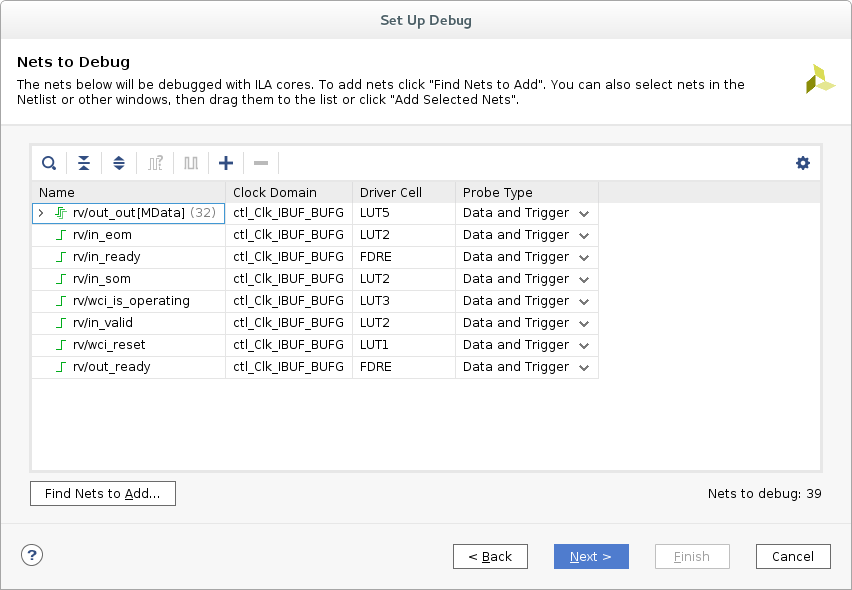
\includegraphics[scale=0.6]			{figures/xilinx_vivado_2017_set_up_debug}}
					\caption{Xilinx Vivado 2017.1 Set Up Debug}
			\end{figure}
		\item Confirm that the debug cores are listed:
			\begin{figure}[H]
				\centerline{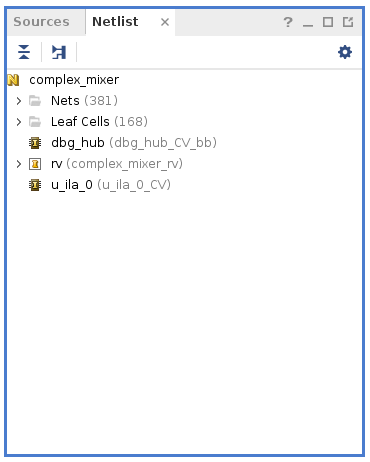
\includegraphics[scale=0.6]			{figures/xilinx_vivado_2017_debug_cores_listed}}
					\caption{Xilinx Vivado 2017.1 Debug Cores Listed}
			\end{figure}
		\item Rerun synthesis. Note that you may once again want to set the \code{flatten\_hierarchy} option set to ``none'' via the GUI. Observe the debug cores in the worker's netlist:
			\begin{figure}[H]
				\centerline{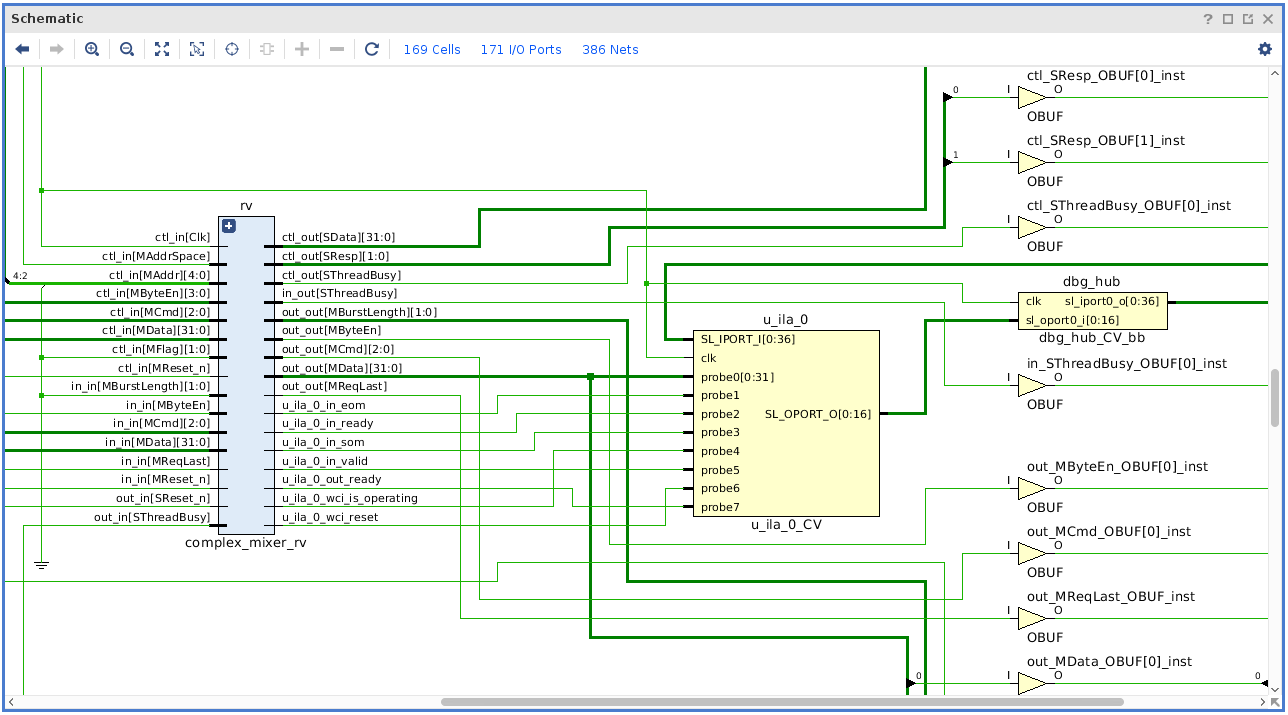
\includegraphics[scale=0.4]			{figures/xilinx_vivado_2017_debug_cores_schematic}}
					\caption{Xilinx Vivado 2017.1 Debug Cores Schematic}
			\end{figure}
		\item Enter the Tcl Console, and overwrite the netlist created by the `make' system in the ``target-zynq'' directory:
			\subitem \code{> write\_edif -security\_mode all -force complex\_mixer.edf}
			\subitem \textit{Note:} ``-force'' tells the write\_edif command to overwrite the file if it already exists.
			\subitem \textit{Note:} ``-security\_mode all'' ensures that partially encrypted designs will still result in a single EDIF file.
		\item In the Tcl Console, generate the *.ltx file containing the debug probe information:
			\subitem \code{> write\_debug\_probes complex\_mixer.ltx}
		\item Build an HDL assembly containing this worker
	\end{enumerate}
The generated bitstream contains the debug and ILA cores which will be recognized by Xilinx Vivado Integrated Logic Analyzer tool. Once the bitstream has been loaded onto the target FPGA, the Analyzer tool can connect and detect the presence of the debug core(s).\newline

\textbf{Reiterating an Important Note for Case 2:} Rebuilding or cleaning the worker (or other AV asset) at any time (with ``make'') will remove any debug functionality added to the Vivado project. The Vivado project files are an artifact of the ``make'' process, and will be overwritten each time ``make'' is run for that asset.


\subsection{Xilinx ISE}
	\subsubsection{Case 1: Integrate ChipScope into HDL Worker using cores from ISE's CORE Generator}
\label{ise1}
		This case assumes that the developer has created a Xilinx CORE Generator project and configured the \textit{Debug and Verification} cores as desired. Specifically, these instructions have been verified for the ICON, ILA and VIO cores. Of the many output files generated by CORE Generator for each core, only two (*.vhd, *.ngc) are necessary to be retained for building the HDL worker and subsequently, the HDL assembly.

		\begin{enumerate}
			\item Integrate the \textit{Debug and Verification} cores into the worker's VHDL:
				\subitem - Declare and instantiate the component for each core (ICON, ILA, VIO, etc)
				\subitem - As needed, add signal declarations and assignments (CONTROL(35 downto 0), TRIG(Y downto 0), DATA(Z downto 0), etc)
			\item Edit the worker's \code{Makefile} to include the path and file name of the
			instantiated cores (ICON, ILA, VIO, etc) *.vhd files. Use the framework's Makefile
			variable ``SourceFiles='' to include the path and name of the VHDL file of each core.
			Absolute or relative paths are acceptable. An example is provided:
			\small\begin{verbatim}
				SourceFiles=../../chipscope/icon1.vhd ../../chipscope/ila_trig32_data128_16384.vhd
			\end{verbatim}
		 	\item Edit the HDL Assembly's \code{Makefile} to include the path and file name of
		 	the	instantiated cores (ICON, ILA, etc) *.ngc files. Use the framework's
		 	Makefile variable ``Cores='' to include the path and name of the NGC file of each
		 	core. Absolute or relative paths are acceptable. An example is provided:
		 	\small\begin{verbatim}
		 		Cores=../../../../components/dsp_comps/cic_dec.hdl/chipscope/icon1.ngc
		 		../../../../components/dsp_comps/cic_dec.hdl/chipscope/ila_trig32_data128_16384.ngc
		 	\end{verbatim}
		 	\item Build HDL worker for target.
			\item Build HDL assembly for platform.
		\end{enumerate}

		The generated bitstream contains the \textit{Debug and Verification} cores which will be recognized by the Xilinx ChipScope Pro Analyzer tool. Once the bitstream has been loaded onto the target FPGA, the Analyzer tool can connect and detect the presence of the \textit{Debug and Verification} core(s).

	\newpage

	\subsubsection{Case 2: Integrate ChipScope into HDL Assembly using the Inserter tool}

		\begin{enumerate}
			\item If the HDL assembly has already been built, proceed to step 2. Otherwise start the
			the HDL assembly build process. Once the build process has completed the \textit{ngdbuild} step, the build process can be canceled.
			\item Launch the Xilinx ChipScope Pro \textit{Inserter} tool and create a new project.
				\subitem Note: The versions of the \textit{Inserter} and \textit{Analyzer} tools must match.
			\item Select the \textit{Input Design Netlist} by browsing to the HDL assembly's container's target directory and selecting the {}-b.ngc file: A example is provide:
				\small\begin{verbatim}
					/data/ocpi_baseassets/ocpiassets/applications/FSK/assemblies/fsk_filerw/
					container-fsk_filerw_matchstiq_base/target-zynq/fsk_filerw_matchstiq_base-b.ngc
			 	\end{verbatim}
			\item The default name and location of the \textit{Output Design Netlist} is acceptable.
			\item The default name and location of the \textit{Output Directory} is acceptable.
			\item Save the project file. When selecting a location to save the project file, it is recommended to not save project in an OpenCPI artifact directory, as they are deleted upon execution of a \textit{make clean} process.
			\item Continue with the Inserter tool process to:
				\subitem - Add signals that are to be monitored
				\subitem - Generate the cores and NGO file:
				\subsubitem - The output folders and files will be generate in \textit{Output Directory} directory.
					\small\begin{itemize}
						\item cs\_icon\_pro/
						\item cs\_ila\_pro\_0/
						\item dump.xst/
						\item fsk\_filerw\_matchstiq\_base-b.ngo
						\item icon\_pro.ngc
						\item ila\_pro\_0.ngc
					\end{itemize}
			\item Used the NGO file to regenerate the NGD
				\subitem i) - Replace the NGC with the NGO by copying *-b.ngo over *-b.ngc.
				\subitem ii) - Rebuild the NGD file based upon \textit{ngdbuild.out}.
					\subsubitem  Within the container's target directory, open the \textit{ngdbuild.out} file and locate the \textit{ngdbuild} command including all of its options necessary for execution. Note that the command in \textit{ngdbuild.out} provides a relative path for ngdbuild. Copy the \textit{ngdbuild} command, modify the command to include the full path to ngdbuild, and execute it from the container's target directory. An example is provided below. Note that this should not be executed from a shell where a Xilinx settings32.sh or settings64.sh script has been sourced.

			\scriptsize\begin{verbatim}
			/opt/Xilinx/14.7/ISE_DS/ISE/bin/lin64/ngdbuild -verbose -uc
					/data/ocpi_baseassets/ocpiassets/applications/FSK/assemblies/../../../hdl/platforms/matchstiq/lib/matchstiq.ucf -p xc7z020-1-clg484 -sd
		 ../../../../../../hdl/platforms/matchstiq/lib/hdl/zynq -sd
		 ../../../../../../hdl/platforms/matchstiq/lib/hdl/zynq -sd
		 ../../../../../../../../ocpi_baseproject/exports/lib/devices/hdl/zynq -sd ../../lib/hdl/zynq -sd
		 ../../../../../../components/dsp_comps/complex_mixer.hdl/chipscope -sd
		 ../../../../../../components/dsp_comps/complex_mixer.hdl/chipscope -sd
		 ../../../../../../../../ocpi_baseproject/exports/lib/adapters/hdl/zynq -sd
		 ../../../../../../components/util_comps/lib/hdl/zynq -sd
		 ../../../../../../components/dsp_comps/lib/hdl/zynq -sd
		 ../../../../../../components/dsp_comps/lib/hdl/zynq -sd
		 ../../../../../../components/dsp_comps/lib/hdl/zynq -sd
		 ../../../../../../components/dsp_comps/lib/hdl/zynq -sd
		 ../../../../../../components/dsp_comps/lib/hdl/zynq -sd
		 ../../../../../../components/dsp_comps/lib/hdl/zynq -sd
		 ../../../../../../../../ocpi_baseproject/exports/lib/adapters/hdl/zynq -sd
		 ../../../../../../../../ocpi_baseproject/exports/lib/devices/hdl/zynq -sd
		 ../../../../../../../../ocpi_baseproject/exports/lib/components/hdl/zynq
		 fsk_filerw_matchstiq_base-b.ngc fsk_filerw_matchstiq_base.ngd
			\end{verbatim}

				\normalsize

			\item Continue the HDL Assembly build process.
				\subitem - Change from the container target directory back to the assembly directory and re-run make
		\end{enumerate}

		The generated bitstream contains the \textit{Debug and Verification} cores which will be recognized by the Xilinx ChipScope Pro Analyzer tool. Once the bitstream has been loaded onto the target FPGA, use the Analyzer tool can connect and detect the presence of the \textit{Debug and Verification} core(s). The saved project file can be imported to automatically populates the names of the signals being monitored.

\newpage

\subsection{Altera}
	\subsubsection{Limitations}
	In versions of Quartus after 14.1, the OpenCPI build flow of exporting QXPs and including SignalTap at the Worker level causes a build failure. Per Altera's website, you can force Quartus to use the legacy SignalTap flow. More details can be found here: \begin{verbatim}https://www.altera.com/support/support-resources/knowledge-base/solutions/rd07012015_904.html\end{verbatim}
	In order to use this build flow, the file /opt/opencpi/cdk/include/hdl/quartus.mk must be modified. An example diff of the change needed can be seen below:
	\scriptsize\begin{verbatim}
	<  ) > $(Core).qsf; echo fit_stratixii_disallow_slm=On > quartus.ini;
---
>  ) > $(Core).qsf; echo fit_stratixii_disallow_slm=On > quartus.ini; echo sci_use_legacy_sld_flow=On >> quartus.ini;
	\end{verbatim}\normalsize
	\subsubsection{Case 1: Integrate SignalTap into HDL Worker using Megafunction cores}
	This case assumes that the developer has created a Quartus IP Parameter Editor project and configured the desired \textit{Altera SignalTap II Logic Analyzer} cores as necessary. Specifically, these instructions have been verified for the sld\_signaltap core. Of the many output files generated by IP Parameter Editor, only one (*.v) is necessary to be retained for building the HDL worker and subsequently, the HDL assembly.
		\begin{enumerate}
			\item Integrate the \textit{Debug and Verification} cores into the worker's VHDL:
				\subitem - Declaration and instantiate the component for the core
				\subitem - As needed, add signal declarations and assignments (acq\_clk, acq\_data\_in(Y downto 0), acq\_trigger\_in(Z downto 0), etc)
			\item Edit the Worker's \code{Makefile} to include the path and file name of the instantiated core *.v files Use the framework's Makefile variable ``SourceFiles='' to include the path and	name of the Verilog file of the core. Absolute or relative paths are acceptable. An example is provided:
			\small\begin{verbatim}
				SourceFiles=./signaltap/sld_trig64_data64_4096.v
			\end{verbatim}
		 	\item Build HDL worker for target.
		 	\item Generate SignalTap format file using Quartus GUI
		 		\subitem - Start Quartus and open the Quartus Project File (.qpf) which is located in the built Worker's target-stratix4 directory. Click File - Create/Update - Create Signal Tap II file from Design Instance(s) and save the file.
			\item Build HDL assembly for platform.
		\end{enumerate}

		The generated bitstream contains the \textit{Debug and Verification} cores which will be recognized by the Altera Quartus SignalTap II Logic Analyzer tool. The executable for this tool (quartus\_stpw) is located with all of the Quartus tools. Once the bitstream has been loaded onto the target FPGA, use the tool can connect and detect the presence of the \textit{Debug and Verification} core(s).
\end{flushleft}


\begin{flushleft}
\end{flushleft}
\newpage


\end{document}
